\documentclass{moderncv}

\moderncvtheme{classic} 
\moderncvcolor{blue}

\definecolor{dark-gray}{gray}{0.20}
                                
\usepackage[utf8]{inputenc}                      
\usepackage[scale=0.75]{geometry}
\usepackage{import}
\usepackage{multicol}
\usepackage{graphicx}
\usepackage{float}
\usepackage[absolute,overlay]{textpos}
\usepackage{lipsum}
\usepackage{etoolbox}
\usepackage[T1]{fontenc}
\usepackage{xcolor}
\usepackage{fontawesome}
\usepackage{fontspec}
\usepackage{color}
\usepackage{tikz}
\usepackage{xpatch}
\usepackage{color,soul}

\usetikzlibrary{shapes.misc,shadows}
\usetikzlibrary{calc,shapes}

\setul{0.5ex}{0.2ex}
\definecolor{Blue}{rgb}{0,0.0,1}
\setulcolor{Blue}

\name{\LARGE{\textcolor{blue}{\textsc{PRASHANT}}}}{\LARGE{\textcolor{blue}{\textsc{KUMAR}}}} 
\address{Ejipura Karnataka, India}{Bengaluru - 560047}
\social[linkedin]{prashantcse}
\phone[mobile]{\faMobilePhone \hspace{7pt}+(91) - 9694725810} 
\social[github]{PrashantPST}
\email{prashantkr.kumar88@gmail.com}


\renewcommand*{\mobilephonesymbol}{}
\renewcommand*{\cventry}[7][.25em]{%
  \cvitem[#1]{#2}{%
    {\bfseries#3}%
%   \ifthenelse{\equal{#4}{}}{}{, {\slshape#4}}% I changed this line (with comma) ...
    \ifthenelse{\equal{#4}{}}{}{ {\slshape#4}}% ... into this one (without comma).
    \ifthenelse{\equal{#5}{}}{}{ {\slshape#5}}%
    \ifthenelse{\equal{#6}{}}{}{ {\slshape#6}}%
    .\strut%
    \ifx&#7&%
      \else{\newline{}\begin{minipage}[t]{\linewidth}\small#7\end{minipage}}\fi}}
            
\begin{document}

\makecvtitle

\section{\textsc{Snapshot}}

\vspace{2pt}

\small{A software engineer currently engaged with Milvik Technology Services India Pvt Ltd having one year and eight months of professional experience. An engineering professional with a Master’s Degree focused in Computer Science \& Engineering from Malaviya National Insitute of Technology Jaipur.}

\vspace{4pt}

\section{\textsc{Work Experience}}

\cventry{Feb 2018--Present}{Software Engineer}{MILVIK India}{}
\small{\begin{itemize}
\item{\ul{L2 Support Month End Automation -}}\\
A web application developed for providing a dashboard for an L2 support team for their month-end tasks.
\begin{itemize}
\item Used Django for backend service and its templating engine for UI rendering.
\item Remove the manual procedures which were error prone.
\item It reduces the time from many hours to just a few minutes.
\item All database operations ran in a transaction; no inconsistent
state of the database even in case of application failure.
\end{itemize}
\item{\ul{Data Migration Service -}}\\
Migration service, a service which was one of the services in a stack of spring-backend microservices.
\begin{itemize}
\item A spring boot enabled service integrated with Kafka.
\item A producer-consumer model where producer listens to the table on one of legacy data source and consumer consumes the same and stores at another data source of the platform databases.
\item The producer was Maxwell’s daemon, an application that reads MySQL binlogs and writes row updates to Kafka.
\end{itemize}
\item{\ul{Data Migration -}}\\
An in-house Python solution for one shot Data Migration.
\begin{itemize}
\item An Extract, Transform \& Load (ETL) approach
\item Extract - mysqlclient, Transform - python script, Load - mysqlclient
\end{itemize}
\end{itemize}}
\vspace{5pt}

\cventry{Nov 2017--Jan 2018}{Software Engineer Trainee}{CodeHall Technology Pvt. Ltd. Bengaluru}{}
\small{\begin{itemize}
\item{\ul{College Connect -}}\\
A web app for helping users(with varied roles) from the beginning of searching colleges to their seat allocation and college orientation for the students of different disciplines.
\begin{itemize}
\item Django backed microservice architecture in conjunction with React for UI.
\item Discuss the Database and API design of each service built by team members.
\item Code develop for StudentProfile and News\&Events services.
\end{itemize}
\end{itemize}}

\thispagestyle{empty} 

\section{\textsc{Projects}}

\vspace{3pt}

\begin{itemize}

\item{\textbf{A Blog Web App}} 
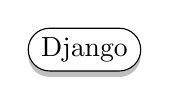
\begin{tikzpicture}[baseline=(char.base)]
\node(char)[draw,fill=white,
  shape=rounded rectangle,
  drop shadow={opacity=.5,shadow xshift=0pt},
  minimum width=0.7cm]
  {Django};
\end{tikzpicture}
\vspace{3pt}

A web application where registered users can write their blog and could post it. Any anonymous user can view all blogs and could also filter blogs for a specific user. A registered user could modify/ delete their blog only. 

\vspace{2pt}

Repo Link: \url{https://github.com/PrashantPST/django-blog.git}

\vspace{3pt}

\item{\textbf{Swiss Tournament}} 
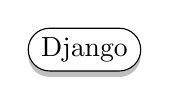
\begin{tikzpicture}[baseline=(char.base)]
\node(char)[draw,fill=white,
  shape=rounded rectangle,
  drop shadow={opacity=.5,shadow xshift=0pt},
  minimum width=0.7cm]
  {Django};
 
\end{tikzpicture}

\begin{tikzpicture}[baseline=(char.base)]
\node(char)[draw,fill=white,
  shape=rounded rectangle,
  drop shadow={opacity=.5,shadow xshift=0pt},
  minimum width=0.7cm]
  {React};
\end{tikzpicture}
\vspace{3pt}

In the Swiss tournament, any player never gets eliminated. Instead, Everyone gets paired in a subsequent round based on their scores. The two closest score player would clash for the next round, and the winner is the one who earns the most points at the end of the tournament.

\vspace{2pt}

Front End Repo: \url{https://github.com/PrashantPST/swiss-tournament-frontend.git}

\vspace{1pt}

Back End Repo: \url{https://github.com/PrashantPST/swiss-tournament-backend.git}

\vspace{3pt}


\item{\textbf{Master's Thesis} SAFETY: Early Detection \& Mitigation of TCP
SYN Flood Utilizing Entropy in Software Defined Networking.

\vspace{3pt}

\small{The thesis presents SAFETY, a novel solution for the early detection and mitigation of TCP SYN flood harnessing the programming and wide visibility approach of SDN using entropy for destination IP with the attribute of TCP flags.}}

\vspace{4pt}

\end{itemize}

\vspace{2pt}

\section{\textsc{Publication}}

\vspace{2pt}

\begin{itemize}
\item{\textbf{SAFETY}: Early Detection and Mitigation of TCP SYN Flood Utilizing Entropy in SDN}\\
\textbf{Publication/Publisher} - IEEE Transactions on Network and Service Management \\
\textbf{Publication date} - 2018-07-31 \\
\textbf{Publication URL} - \url{https://ieeexplore.ieee.org/abstract/document/8423699/}
\end{itemize}

\section{\textsc{Technical Stack}}

\vspace{2pt}

\begin{itemize}

\item \textbf{Programming Language:} 
\begin{tikzpicture}[baseline=(char.base)]
\node(char)[draw,fill=white,
  shape=rounded rectangle,
  drop shadow={opacity=.5,shadow xshift=0pt},
  minimum width=0.7cm]
  {Java};
\end{tikzpicture}

\begin{tikzpicture}[baseline=(char.base)]
\node(char)[draw,fill=white,
  shape=rounded rectangle,
  drop shadow={opacity=.5,shadow xshift=0pt},
  minimum width=0.7cm]
  {Python};
\end{tikzpicture}
\vspace{3pt}
\item \textbf{Web Framework:}
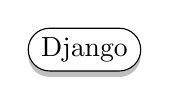
\begin{tikzpicture}[baseline=(char.base)]
\node(char)[draw,fill=white,
  shape=rounded rectangle,
  drop shadow={opacity=.5,shadow xshift=0pt},
  minimum width=0.7cm]
  {Django};
\end{tikzpicture}

\begin{tikzpicture}[baseline=(char.base)]
\node(char)[draw,fill=white,
  shape=rounded rectangle,
  drop shadow={opacity=.5,shadow xshift=0pt},
  minimum width=0.7cm]
  {Spring Boot};
\end{tikzpicture}

\vspace{3pt}

\item \textbf{JavaScript Library}

\begin{tikzpicture}[baseline=(char.base)]
\node(char)[draw,fill=white,
  shape=rounded rectangle,
  drop shadow={opacity=.5,shadow xshift=0pt},
  minimum width=0.7cm]
  {React};
\end{tikzpicture}

\vspace{3pt}

\item \textbf{Database:} 

 \vspace{1pt}
    \begin{itemize}
    \item \textbf{Relational:} 
\begin{tikzpicture}[baseline=(char.base)]
\node(char)[draw,fill=white,
  shape=rounded rectangle,
  drop shadow={opacity=.5,shadow xshift=0pt},
  minimum width=0.7cm]
  {MySQL};
\end{tikzpicture}
\vspace{2pt}
\item \textbf{Document:} 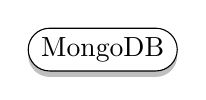
\begin{tikzpicture}[baseline=(char.base)]
\node(char)[draw,fill=white,
  shape=rounded rectangle,
  drop shadow={opacity=.5,shadow xshift=0pt},
  minimum width=0.7cm]
  {MongoDB};
\end{tikzpicture}
    \end{itemize}
    
\vspace{3pt}

\item \textbf{Streaming Platform:} 
\begin{tikzpicture}[baseline=(char.base)]
\node(char)[draw,fill=white,
  shape=rounded rectangle,
  drop shadow={opacity=.5,shadow xshift=0pt},
  minimum width=0.7cm]
  {Apache Kafka};
\end{tikzpicture}

\vspace{3pt}

\item \textbf{Version Control System:} 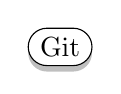
\begin{tikzpicture}[baseline=(char.base)]
\node(char)[draw,fill=white,
  shape=rounded rectangle,
  drop shadow={opacity=.5,shadow xshift=0pt},
  minimum width=0.7cm]
  {Git};
\end{tikzpicture}

\vspace{3pt}

\thispagestyle{empty}

\end{itemize}

\vspace{4pt}

\section{\textsc{Accolades}}

\vspace{1pt}


\begin{itemize}

\item Secured AIR 653 in GATE 2015.

\end{itemize}

\section{\textsc{Education}}

\vspace{3pt}

\begin{itemize}

\item[]{\cventry{2015--2017}{M.Tech. in Computer Engineering}{Malaviya National Institute of Technology}{Jaipur}{7.33 CGPA}{}}

\item[]{\cventry{2010--2014}{B.Tech. in Computer Science \& Engineering}{Govind Ballabh Pant Institute of Engineering \& Technology}{Uttarakhand}{\textit{76.04 \%(Honours)}}{}}

\end{itemize}

\thispagestyle{empty}

\vspace{3pt}



\end{document}